\chapter{Architectural Diagram}
\section{Introduction}
	The Architecture Diagram illustrates the kind of software architecture used to create the system. An architecture allows the way the system functions to be easily understood. Our application’s system uses a client-server architecture, illustrated in the figure below.
\section{Diagram}
\begin{figure}[!ht]
      \centering
      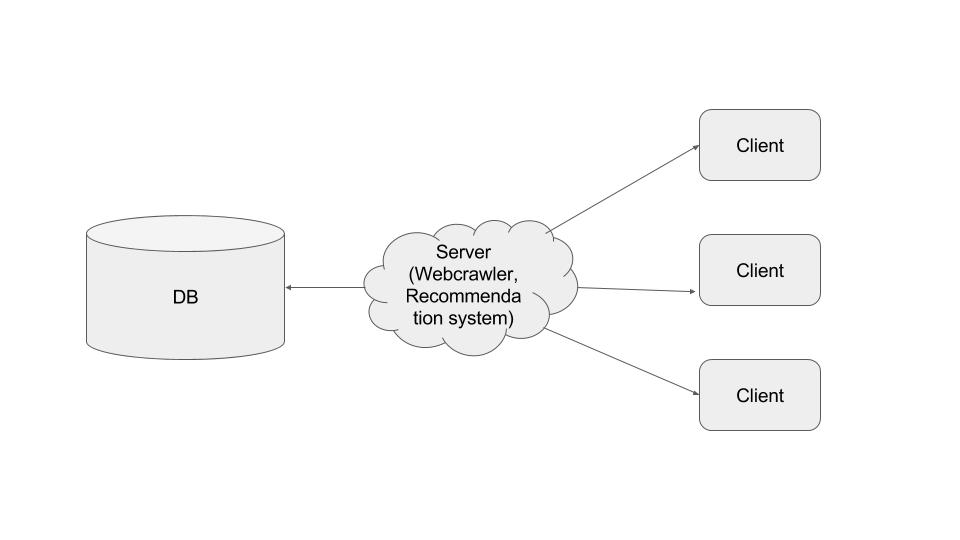
\includegraphics[width=\textwidth]{architecturalDiagram}
      \caption{Architectural Diagram}	
\end{figure}
\section{Architectural Rationale}
	As stated above, our solution uses the client-server architecture. Users, or clients, can access the application through its url. The server then does a lot of the event handling. The server is responsible for having a running web crawler on a cron job that will seek to obtain data, and then index the data appropriately in our real time ElasticSearch database. The server will also be handling the recommendation system as well, so users can have the data they’re customized data. The server will then connect to the database to store the links to the videos ( so we don’t need to actually store massive files). The database will have easily indexable data. 